
%%%%%%%%%%%%%%%%%%%%%%%%%%%%%%%%%%%%%%%%%%%%%%%%%%%%%%%%%%%%%%%%%%%%%%%%%%%%%%%%
%% ************************************************************************** %%
%% *                                Settings                                * %%
%% ************************************************************************** %%
%%%%%%%%%%%%%%%%%%%%%%%%%%%%%%%%%%%%%%%%%%%%%%%%%%%%%%%%%%%%%%%%%%%%%%%%%%%%%%%%
\documentclass{tron}

\loadglsentries{gls}
\glsaddall
\addbibresource{reference}
\usepackage{xcolor}  % Coloured text etc.
% fancy note style
% STYLE NOTES : v2.0
% additional fancy boxes
\usepackage[framemethod=TikZ]{mdframed}
%\usepackage{amsthm}

% gray color indicates [OPTIONAL READING]

%%%%%%%%%%%%%%%%%%%%%%%%%%%%%%
%Note
\newenvironment{note}[3][]{%
	\ifstrempty{#1}%
	{\mdfsetup{%
	frametitle={%
	\tikz[baseline=(current bounding box.east),outer sep=0pt]
	\node[anchor=east,rectangle,fill=#2]
	{\strut Note};}}
	}%
	{\mdfsetup{%
	frametitle={%
	\tikz[baseline=(current bounding box.east),outer sep=0pt]
	\node[anchor=east,rectangle,fill=#2]
	{\strut #1};}}%
	}%
	\mdfsetup{innertopmargin=0pt,skipabove=5pt,linecolor=#2,%
		linewidth=2pt,topline=true,%
		frametitleaboveskip=\dimexpr-\ht\strutbox\relax,
		backgroundcolor={white!90!#2}}
	\begin{mdframed}[]\relax%
	\label{#3}}{\end{mdframed}
}
\Crefname{note}{Note}{notes}

\newcommand{\createnoteenv}[6]{
	\refstepcounter{#6}%
	\ifstrempty{#1}%
	{\mdfsetup{%
	frametitle={%
	\tikz[baseline=(current bounding box.east),outer sep=0pt]
	\node[anchor=east,rectangle,fill=#3]
	{\strut #4~#5};}}
	}%
	{
		\mdfsetup{%
			frametitle={%
				\tikz[baseline=(current bounding box.east),outer sep=0pt]
				\node[anchor=east,rectangle,fill=#3]
				{\strut #4~#5:~#1};
			}
		}%
	}%
	\mdfsetup{innertopmargin=0pt,skipabove=5pt,linecolor=#3,%
	linewidth=2pt,topline=true,%
	frametitleaboveskip=\dimexpr-\ht\strutbox\relax,
	backgroundcolor={white!90!#3}}
	\begin{mdframed}[]\relax%
	\label{#2}
}

%%%%%%%%%%%%%%%%%%%%%%%%%%%%%%
%Definition
\newcounter{definition}[section] \setcounter{definition}{0}
\renewcommand{\thedefinition}{\arabic{section}.\arabic{definition}}
\newenvironment{definition}[2][]{%
	\createnoteenv{#1}{#2}{blue!40}{Definition}{\thedefinition}{definition}%
}{\end{mdframed}}
\newenvironment{definition*}[2][]{%
	\createnoteenv{#1}{#2}{gray!40}{Definition}{\thedefinition}{definition}%
}{\end{mdframed}}
\Crefname{definition}{Definition}{definitions}


%%%%%%%%%%%%%%%%%%%%%%%%%%%%%%
%theoremrem
\newcounter{theorem}[section] \setcounter{theorem}{0}
\renewcommand{\thetheorem}{\arabic{section}.\arabic{theorem}}
\newenvironment{theorem}[2][]{%
	\createnoteenv{#1}{#2}{cyan!40}{Theorem}{\thetheorem}{theorem}%
}{\end{mdframed}}
\newenvironment{theorem*}[2][]{%
	\createnoteenv{#1}{#2}{gray!40}{Theorem}{\thetheorem}{theorem}%
}{\end{mdframed}}
\Crefname{theorem}{Theorem}{theorems}

%%%%%%%%%%%%%%%%%%%%%%%%%%%%%%
%Proof
\newcounter{proof}[section]\setcounter{proof}{0}
\renewcommand{\theproof}{\arabic{section}.\arabic{proof}}
\newenvironment{proof}[2][]{%
	\createnoteenv{#1}{#2}{red!20}{Proof}{\theproof}{proof}%
}{\end{mdframed}}
\newenvironment{proof*}[2][]{%
	\createnoteenv{#1}{#2}{gray!40}{Proof}{\theproof}{proof}%
}{\end{mdframed}}
\Crefname{proof}{Proof}{proofs}


%%%%%%%%%%%%%%%%%%%%%%%%%%%%%%
%Alert
\newcounter{alert}[section]\setcounter{alert}{0}
\renewcommand{\thealert}{\arabic{section}.\arabic{alert}}
\newenvironment{alert}[2][]{%
	\createnoteenv{#1}{#2}{red!80}{Alert}{\thealert}{alert}%
}{\end{mdframed}}
\newenvironment{alert*}[2][]{%
	\createnoteenv{#1}{#2}{gray!40}{Alert}{\thealert}{alert}%
}{\end{mdframed}}
\Crefname{alert}{Alert}{alerts}

%%%%%%%%%%%%%%%%%%%%%%%%%%%%%%
%Answer
\newcounter{answer}[section]\setcounter{answer}{0}
\renewcommand{\theanswer}{\arabic{section}.\arabic{answer}}
\newenvironment{answer}[2][]{%
	\createnoteenv{#1}{#2}{orange!60}{Answer}{\theanswer}{answer}%
}{\end{mdframed}}
\newenvironment{answer*}[2][]{%
	\createnoteenv{#1}{#2}{gray!40}{Answer}{\theanswer}{answer}%
}{\end{mdframed}}
\Crefname{answer}{Answer}{answers}

%%%%%%%%%%%%%%%%%%%%%%%%%%%%%%
%Remark
\newcounter{remark}[section]\setcounter{remark}{0}
\renewcommand{\theremark}{\arabic{section}.\arabic{remark}}
\newenvironment{remark}[2][]{%
	\createnoteenv{#1}{#2}{orange!40}{Remark}{\theremark}{remark}%
}{\end{mdframed}}
\newenvironment{remark*}[2][]{%
	\createnoteenv{#1}{#2}{gray!40}{Remark}{\theremark}{remark}%
}{\end{mdframed}}
\Crefname{remark}{Remark}{remarks}


%%%%%%%%%%%%%%%%%%%%%%%%%%%%%%%
%%Example
%\newcounter{example}[section]\setcounter{example}{0}
%\renewcommand{\theexample}{\arabic{section}.\arabic{example}}
%\newenvironment{example}[2][]{%
%	\createnoteenv{#1}{#2}{blue!40!cyan!20}{Example}{\theexample}{example}%
%}{\end{mdframed}}
%\newenvironment{example*}[2][]{%
%	\createnoteenv{#1}{#2}{gray!40}{Example}{\theexample}{example}%
%}{\end{mdframed}}

%%%%%%%%%%%%%%%%%%%%%%%%%%%%%%
%Algorithm
\newcounter{algo}[section]\setcounter{algo}{0}
\renewcommand{\thealgo}{\arabic{algo}.\arabic{algo}}
\newenvironment{algo}[2][]{%
	\createnoteenv{#1}{#2}{yellow!90!brown!60}{Algorithm}{\thealgo}{algo}%
}{\end{mdframed}}
\newenvironment{algo*}[2][]{%
	\createnoteenv{#1}{#2}{gray!40}{Algorithm}{\thealgo}{algo}%
}{\end{mdframed}}
\Crefname{algo}{Algorithm}{algos}

%%%%%%%%%%%%%%%%%%%%%%%%%%%%%%
% CS480 - Exercise
%\setlength{\parskip}{1cm}
%\setlength{\parindent}{1cm}

%\tikzstyle{titregris} =
%[draw=gray,fill=white, shading = exersicetitle, %
%text=gray, rectangle, rounded corners, right,minimum height=.3cm]
%\pgfdeclarehorizontalshading{exersicebackground}{100bp}
%{color(0bp)=(green!40); color(100bp)=(black!5)}
%\pgfdeclarehorizontalshading{exersicetitle}{100bp}
%{color(0bp)=(red!40);color(100bp)=(black!5)}
%\newcounter{exercise}
%\renewcommand*\theexercise{exercice \textbf{Exercice}~n\arabic{exercise}}
%\makeatletter
%\def\mdf@@exercisepoints{}%new mdframed key:
%\define@key{mdf}{exercisepoints}{%
%\def\mdf@@exercisepoints{#1}
%}
%
%\mdfdefinestyle{theoremstyle}{%
%outerlinewidth=0.01em,linecolor=black,middlelinewidth=0.5pt,%
%frametitlerule=true,roundcorner=2pt,%
%apptotikzsetting={\tikzset{mfframetitlebackground/.append style={%
%shade,left color=white, right color=blue!20}}},
%frametitlerulecolor=black,innertopmargin=1\baselineskip,%green!60,
%innerbottommargin=0.5\baselineskip,
%frametitlerulewidth=0.1pt,
%innertopmargin=0.7\topskip,skipabove={\dimexpr0.2\baselineskip+0.1\topskip\relax},
%frametitleaboveskip=1pt,
%frametitlebelowskip=1pt
%}
%\mdtheorem[style=theoremstyle]{exercise}{\textbf{Exercise}}

\newcounter{exercise}[section]\setcounter{exercise}{0}
\renewcommand{\theexercise}{\arabic{exercise}}
\newenvironment{exercise}[2][]{%
	\createnoteenv{#1}{#2}{gray!40}{Exercise}{\theexercise}{exercise}%
}{\end{mdframed}}
\newenvironment{exercise*}[2][]{%
	\createnoteenv{#1}{#2}{gray!40}{Exercise}{\theexercise}{exercise}%
}{\end{mdframed}}

\Crefname{exercise}{Exercise}{exercises}


%%%%%%%%%%%%%%%%%%%%%%%%%%%%%%
%Examples
% {

%     \section{Theorem and lemma examples with title}
%     \begin{theorem}[Pythagoras' theorem]{theorem:pythagoras}
%     In a right triangle, the square of the hypotenuse is equal to the sum of the squares of the catheti.
%     \[a^2+b^2=c^2\]
%     \end{theorem}
%     In mathematics, the Pythagorean theorem, also known as Pythagoras' theorem (see theorem \ref{theorem:pythagoras}), is a relation in Euclidean geometry among the three sides of a right triangle.
%     
%     \begin{definition}[B\'ezout's identity]{def:bezout}
%     Let $a$ and $b$ be nonzero integers and let $d$ be their greatest common divisor. Then there exist integers $x$ and $y$ such that:
%     \[ax+by=d\]
%     \end{definition}
%     This is a reference to Bezout's lemma \ref{def:bezout}
%     
%     
%     \section{Theorem and proof examples without title}
%     
%     \begin{theorem}[]{theorem:theorem1}
%     There exist two irrational numbers $x$, $y$ such that $x^y$ is rational.
%     \end{theorem}
%     
%     \begin{proof}[]{proof:proof1}
%     If $x=y=\sqrt{2}$ is an example, then we are done; otherwise $\sqrt{2}^{\sqrt{2}}$ is irrational, in which case taking $x=\sqrt{2}^{\sqrt{2}}$ and $y=\sqrt{2}$ gives us:
%     \[\bigg(\sqrt{2}^{\sqrt{2}}\bigg)^{\sqrt{2}}=\sqrt{2}^{\sqrt{2}\sqrt{2}}=\sqrt{2}^{2}=2.\]
%     \end{proof}
%
%     \begin{alert}[]{alert:alert1}
%     If $x=y=\sqrt{2}$ is an example, then we are done; otherwise $\sqrt{2}^{\sqrt{2}}$ is irrational, in which case taking $x=\sqrt{2}^{\sqrt{2}}$ and $y=\sqrt{2}$ gives us:
%     \[\bigg(\sqrt{2}^{\sqrt{2}}\bigg)^{\sqrt{2}}=\sqrt{2}^{\sqrt{2}\sqrt{2}}=\sqrt{2}^{2}=2.\]
%     \end{alert}
%     
%     \begin{remark}[]{alert:alert1}
%     If $x=y=\sqrt{2}$ is an example, then we are done; otherwise $\sqrt{2}^{\sqrt{2}}$ is irrational, in which case taking $x=\sqrt{2}^{\sqrt{2}}$ and $y=\sqrt{2}$ gives us:
%     \[\bigg(\sqrt{2}^{\sqrt{2}}\bigg)^{\sqrt{2}}=\sqrt{2}^{\sqrt{2}\sqrt{2}}=\sqrt{2}^{2}=2.\]
%     \end{remark}
%     
%     
%          \begin{exercise}[]{alert:alert1}
%     If $x=y=\sqrt{2}$ is an example, then we are done; otherwise $\sqrt{2}^{\sqrt{2}}$ is irrational, in which case taking $x=\sqrt{2}^{\sqrt{2}}$ and $y=\sqrt{2}$ gives us:
%     \[\bigg(\sqrt{2}^{\sqrt{2}}\bigg)^{\sqrt{2}}=\sqrt{2}^{\sqrt{2}\sqrt{2}}=\sqrt{2}^{2}=2.\]
%     \end{exercise}
%     
%     \begin{algo}[]{algorithm:alert1}
%     If $x=y=\sqrt{2}$ is an example, then we are done; otherwise $\sqrt{2}^{\sqrt{2}}$ is irrational, in which case taking $x=\sqrt{2}^{\sqrt{2}}$ and $y=\sqrt{2}$ gives us:
%     \[\bigg(\sqrt{2}^{\sqrt{2}}\bigg)^{\sqrt{2}}=\sqrt{2}^{\sqrt{2}\sqrt{2}}=\sqrt{2}^{2}=2.\]
%     \end{algo}
%     
%     \begin{note}[Goal]{pink}{note:goal}
%     If $x=y=\sqrt{2}$ is an example, then we are done; otherwise $\sqrt{2}^{\sqrt{2}}$ is irrational, in which case taking $x=\sqrt{2}^{\sqrt{2}}$ and $y=\sqrt{2}$ gives us:
%     \[\bigg(\sqrt{2}^{\sqrt{2}}\bigg)^{\sqrt{2}}=\sqrt{2}^{\sqrt{2}\sqrt{2}}=\sqrt{2}^{2}=2.\]
%     \end{note}

% }
%\usepackage{lipsum}                     % Dummytext
\usepackage{xargs}                      % Use more than one optional parameter in a new commands
\usepackage[colorinlistoftodos,prependcaption,textsize=normalsize]{todonotes}
%
\newcommandx{\unsure}[2][1=]{\todo[linecolor=red,backgroundcolor=red!25,bordercolor=red,#1]{#2}}
\newcommandx{\change}[2][1=]{\todo[linecolor=blue,backgroundcolor=blue!25,bordercolor=blue,#1]{#2}}
\newcommandx{\info}[2][1=]{\todo[linecolor=OliveGreen,backgroundcolor=OliveGreen!25,bordercolor=OliveGreen,#1]{#2}}
\newcommandx{\improvement}[2][1=]{\todo[linecolor=Plum,backgroundcolor=Plum!25,bordercolor=Plum,#1]{#2}}
\newcommandx{\thiswillnotshow}[2][1=]{\todo[disable,#1]{#2}}
%
\preto\printlistoftodos{
    \listoftodos[Todo List]
}

% EXAMPLES:
    % \todo[inline]{The original todo note withouth changed colours.\newline Here's another line.}
    % \lipsum[11]\unsure{Is this correct?}\unsure{I'm unsure about also!}
    % \lipsum[11]\change{Change this!}
    % \lipsum[11]\info{This can help me in chapter seven!}
    % \lipsum[11]\improvement{This really needs to be improved!\newline\newline What was I thinking?!}
    % \lipsum[11]
    % \thiswillnotshow{This is hidden since option `disable' is chosen!}
    % \improvement[inline]{The following section needs to be rewritten!}
    % \lipsum[11]
    % \newpage
    % \listoftodos[Notes]
%%%  Equation Condition
\newenvironment{eqconditions}
  {\par\vspace{\abovedisplayskip}\noindent\begin{tabular}{>{$}l<{$} @{${}={}$} l}}
  {\end{tabular}\par\vspace{\belowdisplayskip}}
\newenvironment{eqconditions*}
  {\noindent\begin{tabular}{>{$}l<{$} @{${}={}$} l}}
  {\end{tabular}}
%%% introduce 4th depth with \paragraph command
\usepackage{titlesec}
\setcounter{secnumdepth}{4}
\titleformat{\paragraph}
{\normalfont\normalsize\bfseries}{\theparagraph}{1em}{}
\titlespacing*{\paragraph}
{0pt}{3.25ex plus 1ex minus .2ex}{1.5ex plus .2ex}

%%% enumeration reference
% constraint
\newlist{constraint-list}{enumerate}{1}
\setlist[constraint-list,1]{leftmargin=*, label= \Roman*}
\creflabelformat{Constraint}{#2#1#3}
\crefname{constraint-listi}{Constraint}{position}
% criteria
\newlist{criteria-list}{enumerate}{1}
\setlist[criteria-list,1]{leftmargin=*, label= \Roman*}
\creflabelformat{Criterion}{#2#1#3}
\crefname{criteria-listi}{Criterion}{position}
% property
\newlist{property-list}{enumerate}{1}
\setlist[property-list,1]{leftmargin=*, label= \Roman*}
\creflabelformat{Property}{#2#1#3}
\crefname{property-listi}{Property}{position}
% assumption
\newlist{assumption-list}{enumerate}{1}
\setlist[assumption-list,1]{leftmargin=*, label= \Roman*}
\creflabelformat{Assumption}{#2#1#3}
\crefname{assumption-listi}{Assumption}{position}

% custom math command
\newcommand{\unit}[1]{\left[\si{#1}\right]}

% additional math packages
\usepackage{physics}
\usepackage{cancel}

% TODO Flags
\newcommand\TODO[1]{{\textcolor{red}{\textbf{#1}}}}
\newcommand\COMMENT[1]{\hl{#1}}

% Custom Format
% \usepackage{float}
% \usepackage[table]{xcolor}
% \usepackage{soul}
\usepackage{multirow}
\usepackage{caption} 
\captionsetup[table]{skip=3pt}
\captionsetup[figure]{skip=0pt}
\titlespacing*{\section}
{0pt}{10pt}{3pt}
\titlespacing*{\subsection}
{0pt}{8pt}{3pt}
\titlespacing*{\subsubsection}
{0pt}{8pt}{3pt}
%hide the highlight box
\hypersetup{
    colorlinks,
    linkcolor={black!50!black},
    citecolor={black!50!blue},
    urlcolor={black!80!black}
}%hide the highlight box

% table formatting
% \setlength{\arrayrulewidth}{1mm}
% \setlength{\tabcolsep}{18pt}
% \renewcommand{\arraystretch}{2.5}
\usepackage{array}
\newcolumntype{C}[1]{>{\centering\let\newline\\\arraybackslash\hspace{0pt}}m{#1}}

% custom math symbol
%% CS 480 %%
\newcommand{\bm}[1]{\mathbf{#1}}
%%%%%%%%%%%%
\newcommand{\RR}{\mathds{R}}
\newcommand{\Id}{\mathbb{I}}
\newcommand{\NN}{\mathds{N}}
\newcommand{\sign}{\mathop{\mathrm{sign}}}
\newcommand{\diag}{\mathop{\mathrm{diag}}}
\newcommand{\argmin}{\mathop{\mathrm{argmin}}}
\newcommand{\zero}{\mathbf{0}}
\newcommand{\one}{\mathbf{1}}
\newcommand{\av}{\mathbf{a}}
\newcommand{\bv}{\mathbf{b}}
\newcommand{\sv}{\mathbf{s}}
\newcommand{\Xv}{\mathbf{X}}
\newcommand{\Yv}{\mathbf{Y}}
\newcommand{\wv}{\mathbf{w}}
\newcommand{\xv}{\mathbf{x}}
\newcommand{\yv}{\mathbf{y}}
\newcommand{\zv}{\mathbf{z}}
\newcommand{\uv}{\mathbf{u}}
\newcommand{\rv}{\mathbf{r}}
\newcommand{\inner}[2]{\langle #1, #2 \rangle}
\newcommand{\red}[1]{{\color{red}#1}}
\newcommand{\blue}[1]{{\color{blue}#1}}
\newcommand{\magenta}[1]{{\color{magenta}#1}}


\newcommand{\ea}{{et al.}\xspace}
\newcommand{\eg}{{e.g.}\xspace}
\newcommand{\ie}{{i.e.}\xspace}
\newcommand{\iid}{{i.i.d.}\xspace}
\newcommand{\cf}{{cf.}\xspace}
\newcommand{\wrt}{{w.r.t.}\xspace}
\newcommand{\aka}{{a.k.a.}\xspace}
\newcommand{\etc}{{etc.}\xspace}
\newcommand{\sgm}{\mathsf{sgm}}
\newcommand{\Dc}{\mathcal{D}}
\newcommand{\ans}[1]{{\textcolor{orange}{\textsf{Ans}: #1}}}



% extra mod
\newcommand{\mref}[1]{\underline{\textbf{\hypersetup{linkcolor=orange}\Cref{#1}\hypersetup{linkcolor=blue}}}}

%%%%%%%%%%%%%%%%%%%%%%%%%%%%%%%%%%%%%%%%%%%%%%%%%%%%%%%%%%%%%%%%%%%%%%%%%%%%%%%%
% Make sure the following block contains the correct information               %
%%%%%%%%%%%%%%%%%%%%%%%%%%%%%%%%%%%%%%%%%%%%%%%%%%%%%%%%%%%%%%%%%%%%%%%%%%%%%%%%
\reporttitle{ECE 488 - Project 1 \& 2}
% \selfstudy % comment this line if this is not a self study report 
% \employername{Employer Name}
% \employerstreetaddress{Employer Address}
% \employerlocation{City, Provice, Country}
\university{University of Waterloo}
\faculty{Faculty of Engineering}%Faculty of Engineering
\department{}%Department of Systems Design Engineering
\groupnumber{1}
\authornameA{Jianxiang (Jack) Xu}
\studentnumberA{20658861}
\reportdate{\today}
%\confidential{1} % comment this line if this is not a confidential report
%\authorstreetaddress{##}
%\authorlocation{##}
%\authorpostalcode{##}
\useheader % comment this line if no need for header
%%%%%%%%%%%%%%%%%%%%%%%%%%%%%%%%%%%%%%%%%%%%%%%%%%%%%%%%%%%%%%%%%%%%%%%%%%%%%%%%
% end of information block...                                                  %
%%%%%%%%%%%%%%%%%%%%%%%%%%%%%%%%%%%%%%%%%%%%%%%%%%%%%%%%%%%%%%%%%%%%%%%%%%%%%%%%

\begin{document}
%%%%%%%%%%%%%%%%%%%%%%%%%%%%%%%%%%%%%%%%%%%%%%%%%%%%%%%%%%%%%%%%%%%%%%%%%%%%%%%%
%% ************************************************************************** %%
%% *                               Title Page                               * %%
%% ************************************************************************** %%
%%%%%%%%%%%%%%%%%%%%%%%%%%%%%%%%%%%%%%%%%%%%%%%%%%%%%%%%%%%%%%%%%%%%%%%%%%%%%%%%
\maketitle
%%%%%%%%%%%%%%%%%%%%%%%%%%%%%%%%%%%%%%%%%%%%%%%%%%%%%%%%%%%%%%%%%%%%%%%%%%%%%%%%
%% ************************************************************************** %%
%% *                           Table of Contents                            * %%
%% ************************************************************************** %%
%%%%%%%%%%%%%%%%%%%%%%%%%%%%%%%%%%%%%%%%%%%%%%%%%%%%%%%%%%%%%%%%%%%%%%%%%%%%%%%%
% \tableofcontents
%%%%%%%%%%%%%%%%%%%%%%%%%%%%%%%%%%%%%%%%%%%%%%%%%%%%%%%%%%%%%%%%%%%%%%%%%%%%%%%%
%% ************************************************************************** %%
%% *                            List of Figures                             * %%
%% ************************************************************************** %%
%%%%%%%%%%%%%%%%%%%%%%%%%%%%%%%%%%%%%%%%%%%%%%%%%%%%%%%%%%%%%%%%%%%%%%%%%%%%%%%%
% \listoffigures
%%%%%%%%%%%%%%%%%%%%%%%%%%%%%%%%%%%%%%%%%%%%%%%%%%%%%%%%%%%%%%%%%%%%%%%%%%%%%%%%
%% ************************************************************************** %%
%% *                             List of Tables                             * %%
%% ************************************************************************** %%
%%%%%%%%%%%%%%%%%%%%%%%%%%%%%%%%%%%%%%%%%%%%%%%%%%%%%%%%%%%%%%%%%%%%%%%%%%%%%%%%
% \listoftables
%%%%%%%%%%%%%%%%%%%%%%%%%%%%%%%%%%%%%%%%%%%%%%%%%%%%%%%%%%%%%%%%%%%%%%%%%%%%%%%%
%% ************************************************************************** %%
%% *                              MAIN BODY                                 * %%
%% ************************************************************************** %%
%%%%%%%%%%%%%%%%%%%%%%%%%%%%%%%%%%%%%%%%%%%%%%%%%%%%%%%%%%%%%%
\clearpage
\pagenumbering{arabic}
\setcounter{page}{1}
\setlength{\parskip}{5pt}
\newpage

%%%%%%%%%%%%%%%%%%%%%%%%%%%%%%%%%%%
%%%%% Intro.  %%%%%%
%%%%%%%%%%%%%%%%%%%%%%%%%%%%%%%%%%%

%%%%%%%%%%%%%%%%
%%%%% Ex 1 %%%%%
%%%%%%%%%%%%%%%%
\section{Problem P1: Classical design for the SISO aiming system}
\vspace{5pt}

% --- ANS (a) --- %
\subsection{(a) Verify the linearization \label{ans:P1-a}}
	For the given nonlinear motion equations:
	\begin{align}
		& \frac32 \ddot{w} + \frac14 \left[ \ddot{\theta} \cos{(\theta)} - (\dot{\theta})^2 \sin(\theta) \right] = 0 \label{eqn:a:1} \\
		& \frac16 \ddot{\theta} + \frac14 \left[ \ddot{w} \cos{(\theta)} - g \sin(\theta) \right] = \tau \label{eqn:a:2}
	\end{align}
	
	We may linearize \Cref{eqn:a:1} and \Cref{eqn:a:2} about $\theta = 0$ with Taylor series for small angle changes:
	\begin{align}
		& \frac32 \ddot{w} + \frac14 \left[ \quad \ddot{\theta} \, \cancelto{1}{\cos{(\theta)}} \quad  - \cancelto{0}{(\dot{\theta})^2} \, \cancelto{\theta}{\sin(\theta)} \quad \right] = 0  \\
		& \frac16 \ddot{\theta} + \frac14 \left[ \quad  \ddot{w} \, \cancelto{1}{\cos{(\theta)}} \quad  - g \, \cancelto{\theta}{\sin(\theta)} \quad \right] = \tau 
	\end{align}
	
	Hence, we may obtain the linearized set of equations as following:
	\begin{align}
		& \frac32 \ddot{w} + \frac14 \ddot{\theta} = 0 \label{eqn:a:1:linear} \\
		& \frac16 \ddot{\theta} + \frac14 \ddot{w} - \frac14 g \theta = \tau \label{eqn:a:2:linear}
	\end{align}
	
	From \Cref{eqn:a:1:linear}, we may obtain:
	\begin{equation}
		\ddot{w} = -\frac16 \ddot{\theta} \label{eqn:a:w-theta}
	\end{equation}
	
	Substitute \Cref{eqn:a:w-theta} into \Cref{eqn:a:2:linear}, we may obtain:
	\begin{equation}
		\frac16 \ddot{\theta} - \frac1{24} \ddot{\theta} - \frac14 g \theta = \tau \quad \Rightarrow \quad \frac18 \ddot{\theta}- \frac14 g \theta = \tau
	\end{equation}
	
	Applying Laplace transform, we may obtain the transfer function:
	\begin{align}
		\because \qquad 		& \mathcal{L}\left\{ \frac18 \ddot{\theta}- \frac14 g \theta = \tau \right\} \\
		\therefore \qquad 	& \frac18 s^2 \Theta(s) - \frac{g}4 \Theta(s) = \mathbb{T}(s)  \\
		\therefore \qquad 	& P_1 (s) = \frac{\Theta(s)}{\mathbb{T}(s)} = \frac{1}{\frac18 s^2  - \frac{g}4} = \frac{8}{s^2 - 2 g} = \frac{8}{(s - \sqrt{2g})(s + \sqrt{2g})}
	\end{align}
	
	Now, by sub in numerical value $g = 9.8$, and we may obtain a numerical transfer function of the plant $P_1(s)$:

	\begin{note}[Final Linearized Plant $P_1(s)$]{pink}{note:p1}	
		\begin{equation}
			 P_1(s) = \frac{\Theta(s)}{\mathbb{T}(s)} \approx \frac{8}{(s-4.427)(s+4.427)} \label{eqn:p1}
		\end{equation}
	\end{note}
	
	\textbf{Q.E.D.}


% --- ANS (b) --- %
\clearpage
\subsection{(b) Compute $W(s)/\tau(s)$\label{ans:P1-b}}
	Recall \Cref{ans:P1-a}, we obtained the relationship between $w$ and $theta$ in time domain as stated in \Cref{eqn:a:w-theta}. We may apply Laplace transform, and obtain their s-domain relationship:
	\begin{equation}
		\mathbb{W}(s) = - \frac16 \mathbb{T}(s)
	\end{equation}
	
	Hence, we may obtain the transfer function $P_2(s)$:
	
	\begin{note}[Final Linearized Plant $P_2(s)$]{pink}{note:p2}
		\begin{equation}
			P_2(s) = \frac{\mathbb{W}(s)}{\mathbb{T}(s)} = - \frac{1}{6} \frac{\Theta(s)}{\mathbb{T}(s)} \approx - \frac{4/3}{(s-4.427)(s+4.427)}
		\end{equation}
	\end{note}



% --- ANS (c) --- %
\subsection{(c) Classical Control Design \label{ans:P1-c}}
	The goal is to design a controller $C_1(s)$ for the plant $P_1(s)$ such that all three specifications are met:
	\begin{spec-list}
		\item The closed-loop sytem is stable \label{spec:stable}
		\item For step reference signals, the steady-state tracking error $|e_\infty| \leq 10\%$ \label{spec:ess}
		\item The phase margin is at least $50^\circ$ \label{spec:pm}
	\end{spec-list}


	As we may observed from the plant function \Cref{eqn:p1}, there exists a pole in \Gls{ORHP}, hence the closed loop plant is unstable, as observed in the root locus plot and step response in \verb|'sisotool'| (as shown \Cref{fig:siso-p1} below). 
	
	{	
		\centering
      	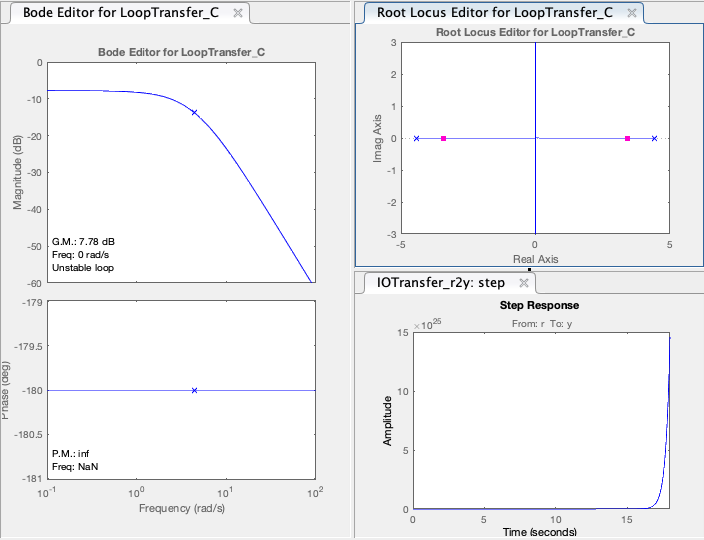
\includegraphics[width=350px]{Fig/sisotool-p1}
      	\captionof{figure}{Control panel view of the SISOtool\label{fig:siso-p1}}
      	\par
    }
    
    Hence, we need a real zero in \Gls{LHP} for the loop gain $L_1(s) = C(s)P_1(s)$. To make the controller proper, we may need an extra pole in $C(s)$. Hence, we may possibly stabilize the $P_1$ plant (\Cref{spec:stable}) with a first order controller. 

	From the bode plot in \Cref{fig:siso-p1}, we may find the DC gain is below $0\unit{dB}$ and the phase plot is a line at $-180^\circ$. Hence, to satisfy \Cref{spec:ess} and \Cref{spec:pm}, we need a lead filter with zero dominant, so that we can pull up the phase margin around the cross-over frequency $w_{cg}$ to obtain proper phase margin.
	
	We shall find the proper gain and zeros first to satisfy the steady state error and phase margin (\Cref{spec:ess} and \Cref{spec:pm}), and then determine the proper pole after the cross over frequency $\omega_{gc}$ to maintain the margin within the \Cref{spec:pm}. 
		
	\begin{note}[Step 1: determine the zero location]{blue!20!white}{p1:c:step1}
		As \Cref{fig:rl-zero} shown below, there are three cases of zero locations so that the closed loop would be stable: zero on the right of the plant \Gls{LHP} pole (Option A), zero on the left of the plant poles (option B), and zero at the \Gls{LHP} plant pole (option C). To note, the zero has to locate in LHP to ensure closed loop stable.
	
		{	
			\centering
	      	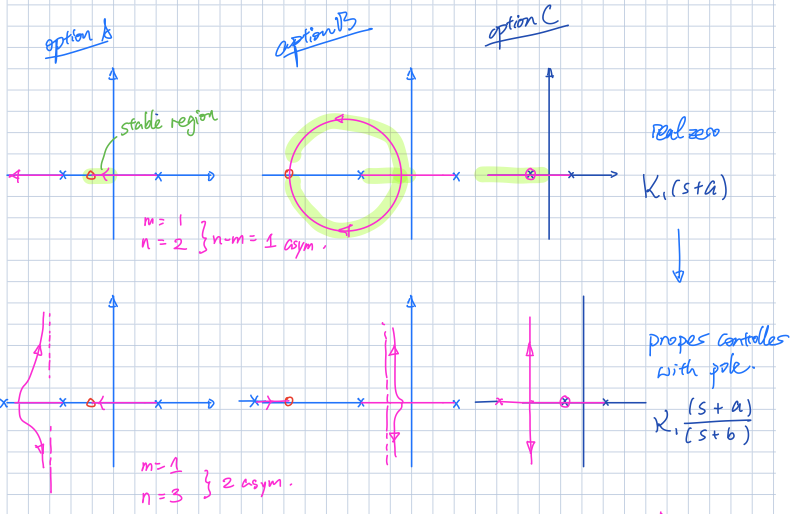
\includegraphics[width=450px]{Fig/root-locus}
	      	\captionof{figure}{Zero placement in root locus\label{fig:rl-zero}}
	      	\par
	    }
	    
	    It is possible to design a proper controller with all three options to stabilize the plant (as required by \Cref{spec:stable}), but there would be pros and cons in each option.
	    
	    For simplicity, we proceed with option C, which results a pole cancellation, resulting a reduced order in the closed-loop. Hence, let $C_1' = K_1 (s+a) = K_1 (s + 4.427)$ with pole at $s = -4.427$.	
	\end{note}
	
	\begin{note}[Step 2: determine the gain]{blue!20!white}{p1:c:step2}
		To satisfy the steady state error (\Cref{spec:ess}), we may determine the minimum gain required:
		\begin{align}
			\left| \frac1{1+P_1(s=0)C_1(s=0)} \right| & \leq e_{ss}^{max} = 10\% \\
			\frac1{1 + \left|\frac{8}{(s-4.427)(s+4.427)}\right| \, K_1 (s + 4.427)}  & \leq 0.1\\
			\frac1{1 + \frac{8 \,  K_1}{4.427}} & \leq 0.1 \\
			9 & \leq \frac{8}{4.427} \, K_1 \\
			4.98 & \leq K_1 
		\end{align}
		
		Hence, we need a minimum of 4.98 as the gain. For simplicity, let's assume $K_1 = 10$, so that we may compensate the later gain loss from the pole.
		
		Now the controller is formulated as:
		\begin{equation}
			C_1(s)' = K_1 (s + a) = 10 (s + 4.427) \label{eqn:c1:gain}
		\end{equation}
	\end{note}
	
	Let's checkout the effect of the current improper controller $C_1'(s)$ designed above. 
	
	{	
		\centering
		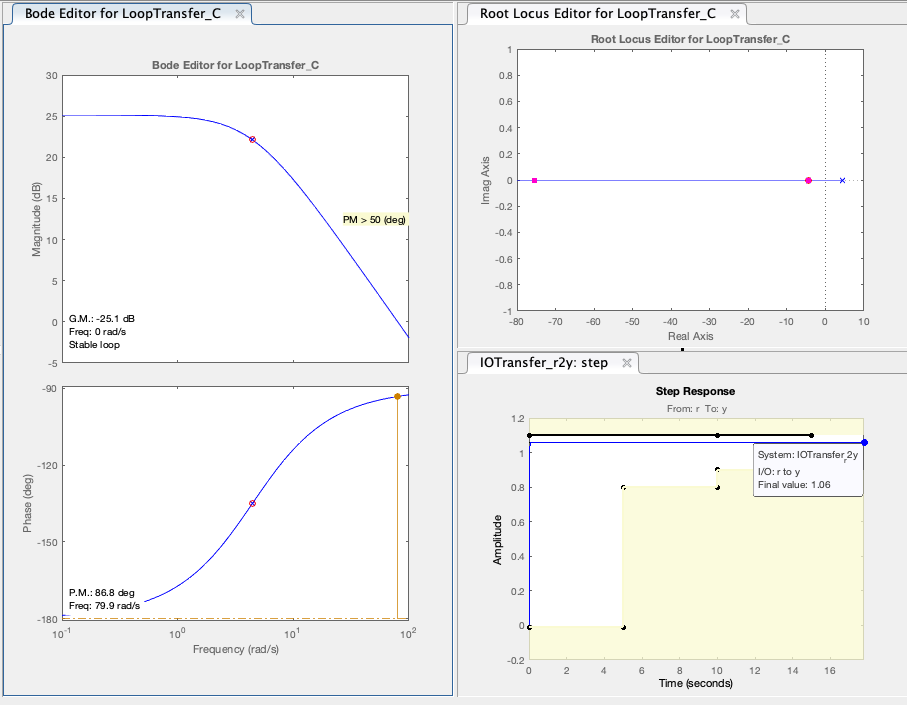
\includegraphics[width=450px]{Fig/sisotool-c1-zero.png}
      	\captionof{figure}{SISO Control Panel of the current design $C_1'(s)$ \label{fig:siso-zero}}
    }
	
	From \Cref{fig:siso-zero}, we may observe we have satisfied the steady state spec \Cref{spec:ess}, and we have also satisfied the phase margin requirement \Cref{spec:pm}. Hence, additional lead compensator is not required. 
	
	\begin{note}[Step 3: determine the pole]{blue!20!white}{p1:c:step3}
		Now, we may determine the pole to make it proper, with $\frac{1}{\tau s + 1}$. 
		
		Ideally, $\tau < \frac{1}{10\, \omega_{gc}} = \frac1{80 \unit{rad/s} \times 10} = 0.00125$ 
		
		Hence, let's use $\tau = 0.001 [s]$.
	\end{note}
	
	As a result, the final controller is:
	
	\begin{note}[Final Controller $C_1(s)$]{pink}{note:c1}
		\begin{equation}
			C_1(s) = \frac{10 (s + 4.427)}{0.001 s + 1} \label{eqn:c1}
		\end{equation}		
	\end{note}

	As observed in SISO tool (as shown in \Cref{fig:siso-c1} below), the controller is stable, the phase margin is $PM=82.3^\circ$ and the steady state error is $|e_{ss}| = 6\%$. Hence, all specs (\Cref{spec:stable}, \Cref{spec:ess}, \Cref{spec:pm}) are met with \Cref{eqn:c1}.
	
	{	
		\centering
		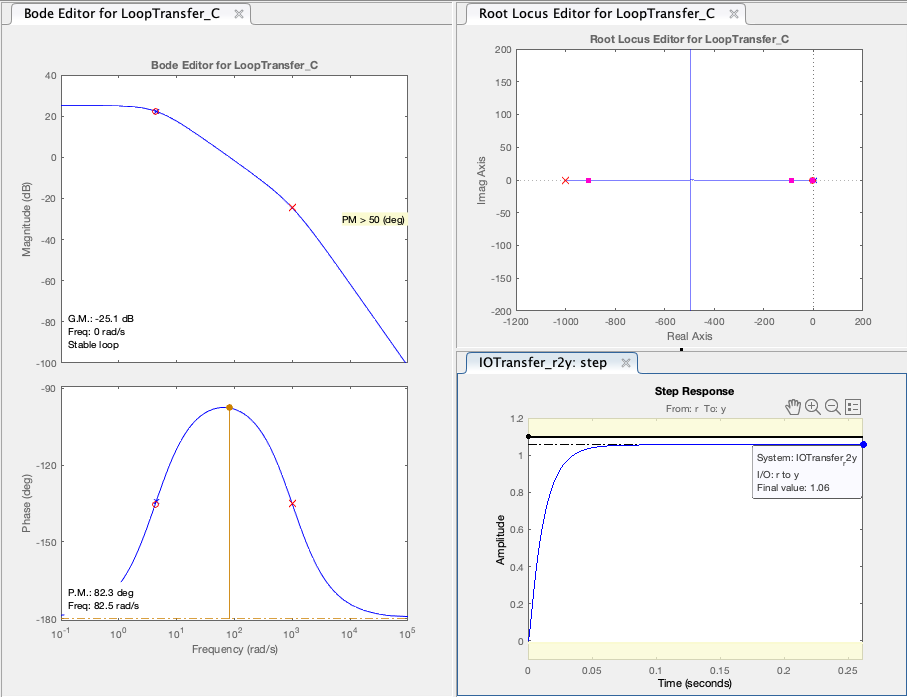
\includegraphics[width=450px]{Fig/sisotool-c1.png}
      	\captionof{figure}{SISO Control Panel of the final controller design $C_1(s)$ \label{fig:siso-c1}}
    }
	
% --- ANS (d) --- %
\subsection{(d) MATLAB : Performance Evaluation \label{ans:P1-d}}
	{	
		\centering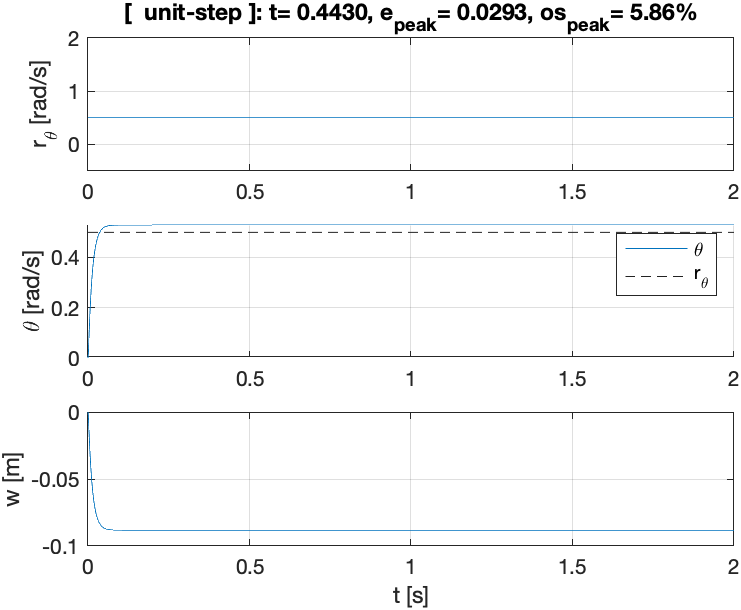
\includegraphics[width=300px]{../matlab/output/q1/step_response_unit-step.png}
      	\captionof{figure}{Closed-loop response for a step input of $0.5 \unit{rad}$  \label{fig:p1:response:0Hz}}
	}
	
	\begin{figure}[h]
		\centering
		\subfloat[$0.5\unit{Hz}$ \label{fig:p1:response:0p5Hz}]{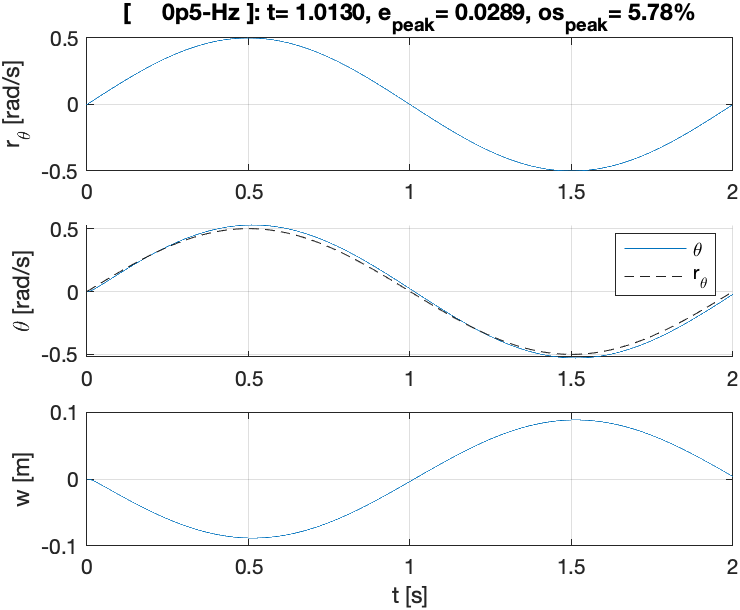
\includegraphics[width=220px]{../matlab/output/q1/step_response_0p5-Hz}}
		\qquad
		\subfloat[$2\unit{Hz}$ \label{fig:p1:response:2Hz}]{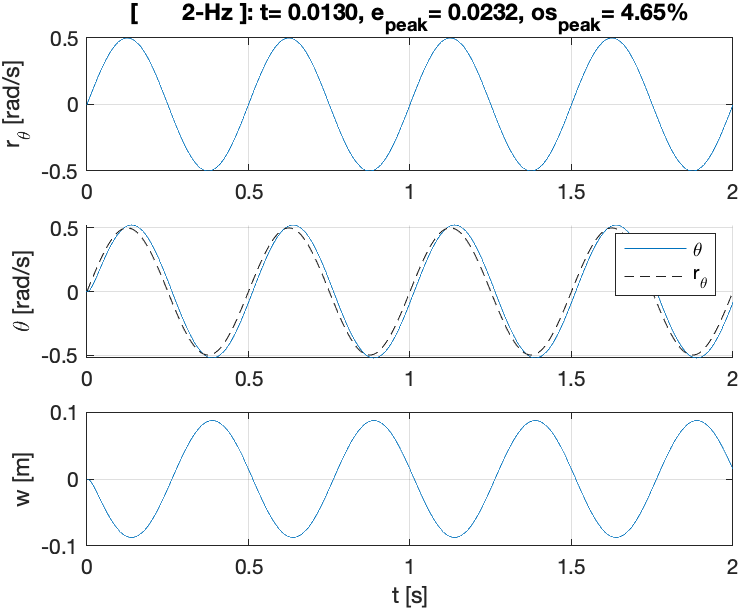
\includegraphics[width=220px]{../matlab/output/q1/step_response_2-Hz}}
		\\
		\subfloat[$10\unit{Hz}$ \label{fig:p1:response:10Hz}]{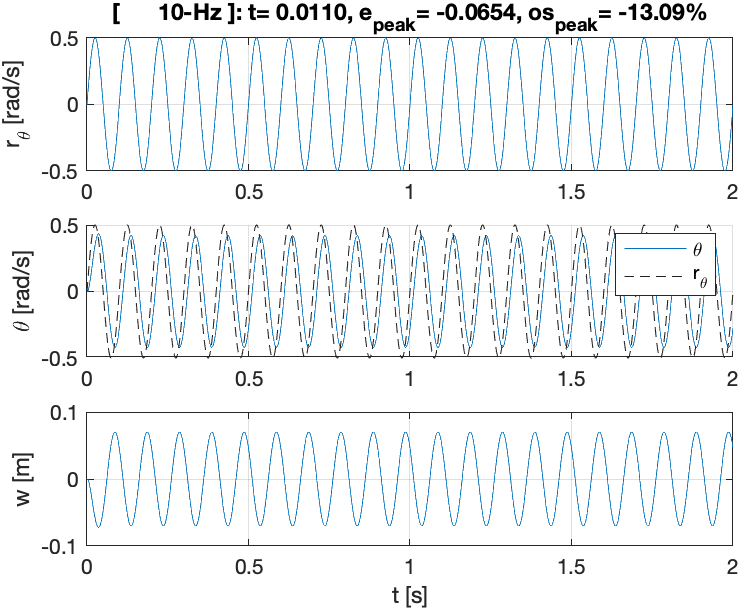
\includegraphics[width=220px]{../matlab/output/q1/step_response_10-Hz}}
		\qquad
		\subfloat[$100\unit{Hz}$ \label{fig:p1:response:100Hz}]{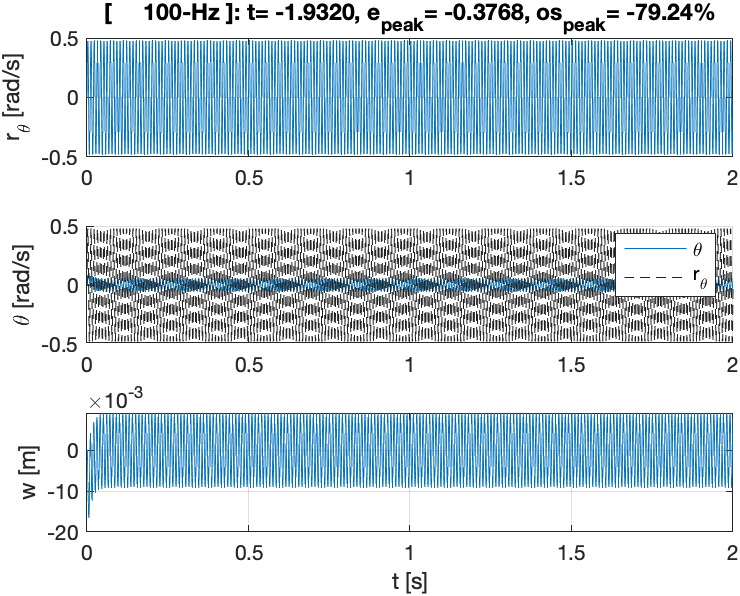
\includegraphics[width=220px]{../matlab/output/q1/step_response_100-Hz}}
		\caption{Closed-loop response for sinusoidal inputs \label{fig:p1:responses}}
	\end{figure}
	
	\clearpage
	\begin{remark}[Steady-state tracking error verification]{}
		As suggested by \Cref{spec:ess}, we shall have a steady state error less than 10\%, it is verified with a unit step input as shown in \Cref{fig:p1:response:0Hz} which has shown the steady state error is less than 5.86\%. To note, the $os_{peak}$ here indicates the percent overshoot from the input peak. Since the system is under-damp as designed, the peak here would be the steady-state value, and the overshoot percentage indicates the steady state error. Hence, we may conclude, the \Cref{spec:ess} has been satisfied, and the controller is indeed stable.
	\end{remark}
	
	\begin{remark}[Comment on the tracking performance for oscillatory signals]{}
		As observed from \Cref{fig:p1:response:2Hz}, it performs the best with smaller steady state error and faster response. In addition, as observed from \Cref{fig:p1:response:0p5Hz}, we also see slight improvements in both steady state error and rise time delay. However, at higher frequency (\Cref{fig:p1:response:10Hz} and \Cref{fig:p1:response:100Hz}), we see the steady state error and rise time delay has been dramatically worsen as the frequency increase. 
		
		This is as what we expected. As the frequency increases, the gain should be attenuated. At the low frequency range, the gain is reduced slightly, whereas the gain is reduced much dramatically at higher frequency after (about 6Hz). We shall expect the peak value reduced and the steady state error enlarged as the frequency increased. As observed, the peak value is reduced throughout all frequency as frequency increased. Since the steady state error was originated from the overshoot of the target value at DC step input, this overshoot would be reduced as the frequency increases at low frequency band, resulting an increased performance in steady state error at low frequency. As observed, the steady state error is reduced slightly in low frequency band and increased dramatically in high frequency band. 
	
		The rise time should improve at low frequency before the crossover frequency $\omega_{gc} = 82.5 \unit{rad/s} = 13.13 [Hz]$, since the phase increases at low frequency band as the frequency increases. The rise time shall be worsen as the frequency continues to increase in high frequency. 
	\end{remark}


	\begin{note}[Optional: Simulation]{blue!40!white}{}
		Thanks to Professor's provided simulation, we may now see how it works! 
		
		(Please enable by \verb|`EN_SIM'|)
		
		{	
			\centering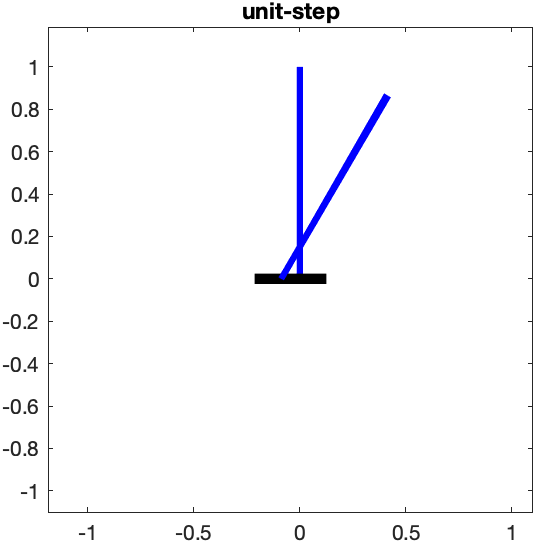
\includegraphics[width=180px]{../matlab/output/q1/sim_unit-step}
	      	\captionof{figure}{Simulation result of unit-step input  \label{fig:p1:sim:0Hz}}
		}
		{	
			\centering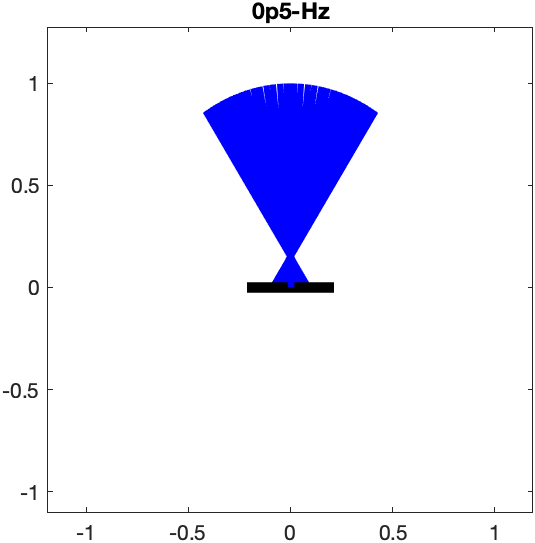
\includegraphics[width=180px]{../matlab/output/q1/sim_0p5-Hz}
	      	\captionof{figure}{Simulation result of sinusoidal input at $0.5\unit{hz}$  \label{fig:p1:sim:0p5Hz}}
		}
		{	
			\centering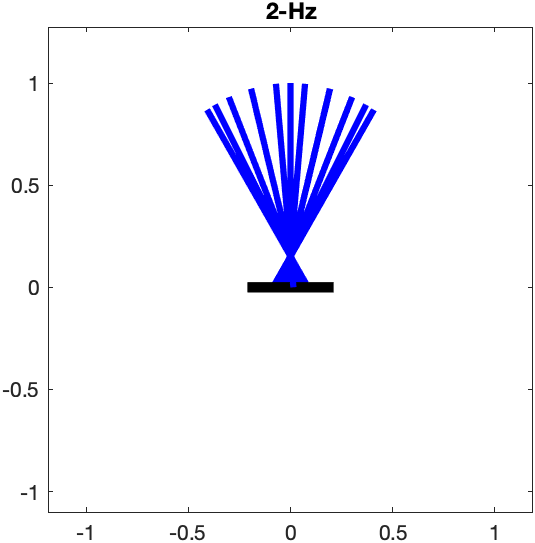
\includegraphics[width=180px]{../matlab/output/q1/sim_2-Hz}
	      	\captionof{figure}{Simulation result of sinusoidal input at $2\unit{hz}$  \label{fig:p1:sim:2Hz}}
		}

	\end{note}


%%%%%%%%%%%%%%%%
%%%%% Ex 2 %%%%%
%%%%%%%%%%%%%%%%
\newpage
\section{Problem P2: Further analysis of the SISO aiming system controller}
\vspace{5pt}

\subsection{(a) Loop Gain $L_1(s) = P_1(s) C_1(s)$ Bode Plot \label{ans:P2-a}}
		{	
			\centering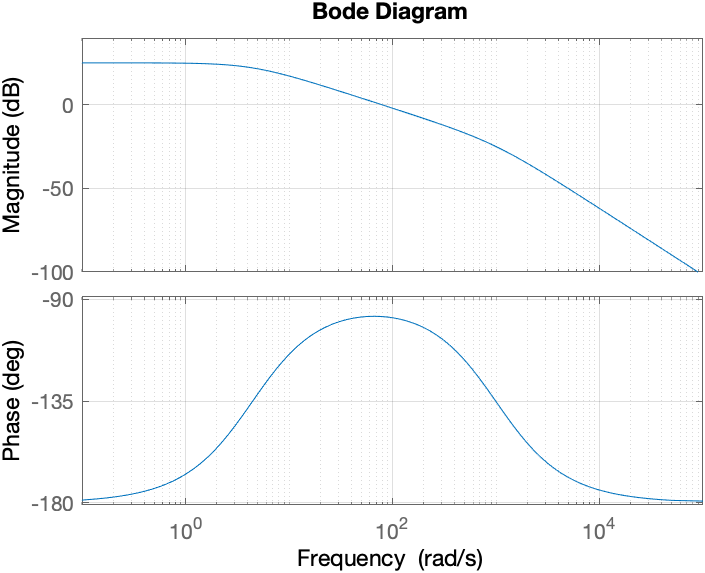
\includegraphics[width=300px]{../matlab/output/q2/bode_plot_L1}
	      	\captionof{figure}{Bode plot of the loop gain ($L_1(s) = P_1(s) C_1(s)$)  \label{fig:p2:a}}
		}
		
		Recall a typical good loopshape has $|L(j\omega)|$ large at low frequencies and small at high frequency. As observed in \Cref{fig:p2:a}, the loop gain indeed appears such characteristic, hence, it is a "typical good loopshape".

\subsection{(b) Bandwidth of the control system \label{ans:P2-b}}
	From the MATLAB function \verb|`bandwidth'|, we obtained the closed loop bandwidth as $BW = 81.93 \unit{rad/s}$. Since the unstable plant pole is located at $p=4.427 \unit{rad/s}$, the rule of thumb is indeed satisfied:
	
	\begin{equation}
		BW = 81.93 \unit{rad/s} \gg 2p = 2 \times 4.427 \unit{rad/s}
	\end{equation}

\newpage
\subsection{(c) Robustness analysis of $C_1(s)$ \label{ans:P2-c}}
	To evaluate the performance of the closed-loop systems for original and modified plant, we shall plot their bode plot and root locus for the open loop, and corresponding closed-loop unit-step response.
	
	{	
		\centering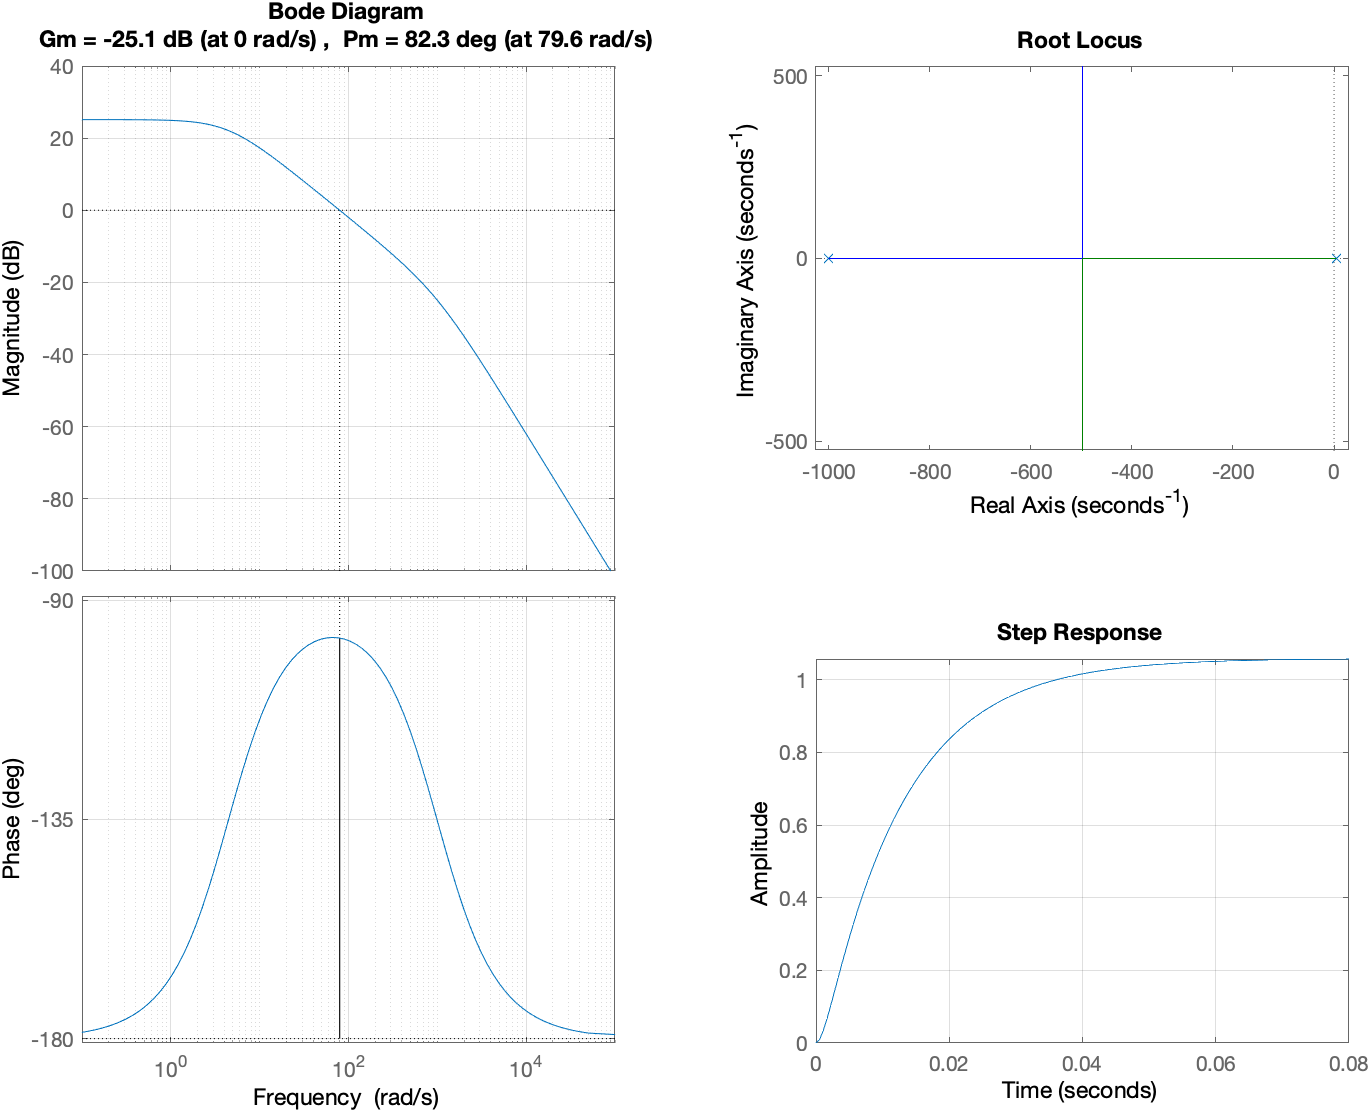
\includegraphics[width=350px]{../matlab/output/q1/siso_plot_L1}
      	\captionof{figure}{Characteristic plots with the original pant ($P_1$)  \label{fig:p2:c:siso-p1}}
	}
		
	{	
		\centering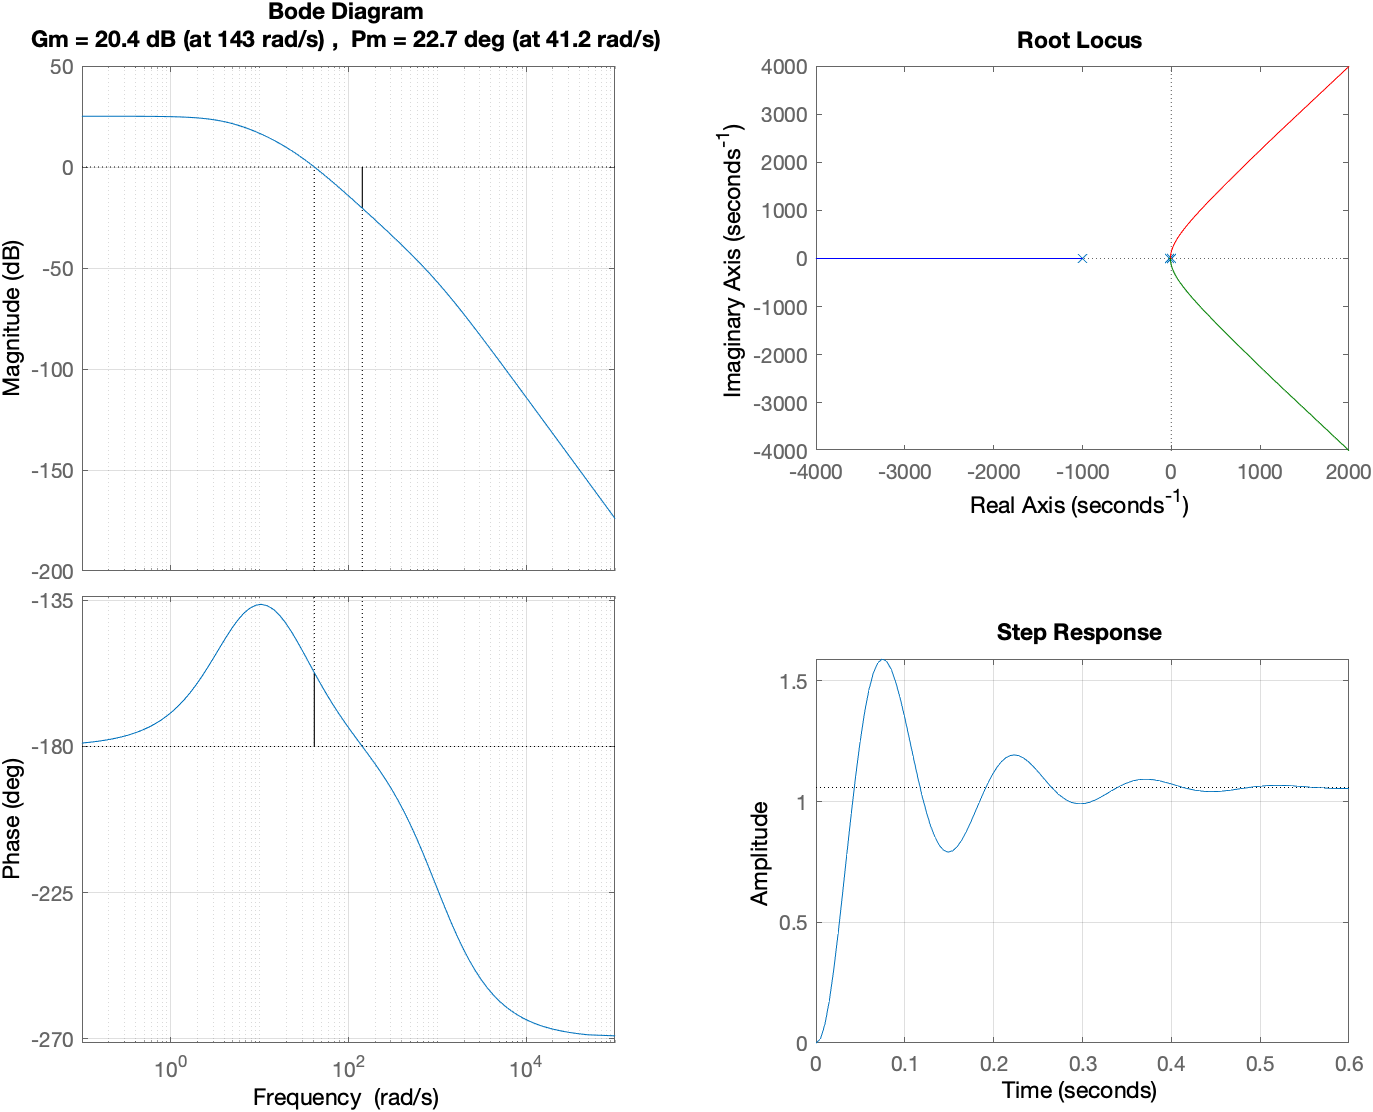
\includegraphics[width=350px]{../matlab/output/q2/siso_plot_p2ci-L1-modified}
      	\captionof{figure}{Characteristic plots with the modified pant ($P_1^{modified}$)  \label{fig:p2:c:siso-p1-mod}}
	}
	
	\clearpage
	\begin{note}[i) Comments on Modified Plant]{pink}{note:p2:i}
		As observed in \Cref{fig:p2:c:siso-p1-mod}, the closed-loop system appear to be stable. The step response (also shown in \Cref{fig:p2:c:p1-mod-response} below) becomes under-damped with some oscillations and significant overshoot (which was not observed in \Cref{fig:p2:c:siso-p1}). The phase margin is reduced significantly from $82 \unit{deg}$ to $23 \unit{deg}$. 
		
		{	
			\centering
			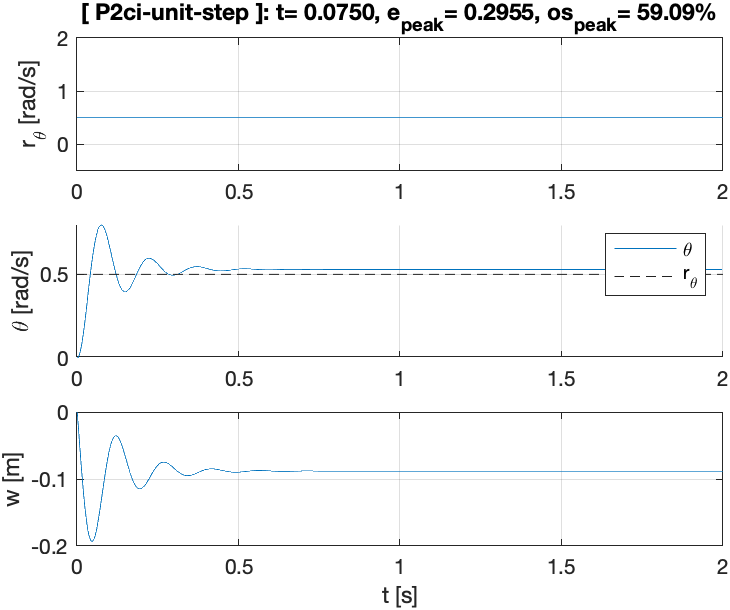
\includegraphics[height=180px]{../matlab/output/q2/step_response_P2ci-unit-step} \qquad
			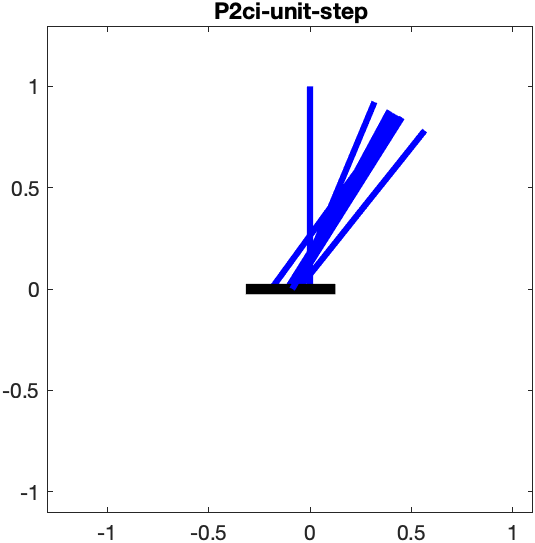
\includegraphics[height=180px]{../matlab/output/q2/sim_P2ci-unit-step}
	      	\captionof{figure}{Unit step response and simulation with the modified pant ($P_1^{modified}$)  \label{fig:p2:c:p1-mod-response}}
		}			
		
		This is as expected with our intuition, since the modified plant introduced another pole at $25 \unit{rad/s}$, which would pull down the the gain and phase before the original crossover frequency ($79.6 \unit{rad/s}$), introducing a significant phase lag to the system. In addition, the extra pole makes the asymptote into complex plane of root-locus, resulting oscillation in the step response. 
	\end{note}
	
	\begin{proof}[ii) The perturbed plant in \Cref{note:p2:i} a particular case of the uncertainty model]{proof:p2}
		Let's say there exist some $\{\Delta(s) : |\Delta(j\omega)| < 1 ,\,\forall \omega \in \mathbb{R^+}\}$, such that $(1 + \Delta(s)W(s)) = \frac{25}{s + 25}$.
		
		\begin{align}
			(1 + \Delta(s)W(s)) &= \frac{25}{s + 25} \\
			\Delta(s) &= \frac{\frac{25}{s + 25} - 1}{W(s)} \\
			\Delta(s) &= - \frac{1}{10} \frac{s+200}{s+25}
		\end{align}
		
		Let's see if the condition ($|\Delta(j\omega)| < 1 ,\,\forall \omega \in \mathbb{R^+}$) still holds:
		
		\begin{align}
			|\Delta(j\omega)| &= \left|- \frac{1}{10} \frac{j\omega+200}{j\omega+25}\right| \\
			\because \qquad & |\Delta(j\omega)|_{\omega\rightarrow\infty} = \left|- \frac{1}{10} \cancelto{1}{\frac{j\omega+200}{j\omega+25}} \right| = 0.1\\
							& |\Delta(j\omega)|_{\omega\rightarrow0} = \left|- \frac{1}{10} \cancelto{1}{\frac{200}{25}} \right| = 0.8\\
			\therefore \qquad & |\Delta(j\omega)| < 1 \forall \omega
		\end{align}
		
		Hence, there indeed exists such $\{\Delta(s) : |\Delta(j\omega)| < 1 ,\,\forall \omega \in \mathbb{R^+}\}$, such that $(1 + \Delta(s)W(s)) = \frac{25}{s + 25}$. 
		
		More specifically, $P_{1,mode}(s) = \frac{25}{s+25} \cdot P_1(s)$ is a particular case of $P_{1,uncertain}(s) = (1 + \Delta(s) W(s))\cdot P_1(s)$, with $\Delta(s) = - \frac{1}{10} \frac{s+200}{s+25}$ for $W(s) = \frac{10s}{s + 200}$		
		
		\textbf{Q.E.D.}
	\end{proof}


	\begin{note}[iii) Small Gain Theorem]{pink}{note:p2:iii}
		For a multiplicative uncertainty model, the Small Gain Theorem can be simplified to the following:
			\qquad The system is robustly stable, if $|M(j\omega)| = |\frac{L_1(s) W(s)}{1 + L_1(s)}|_{s=j\omega} \leq 1 \, \forall \omega$
			
		Hence, we just need to plot the bode-plot of the transfer function $M(s) = \frac{L_1(s) W(s)}{1 + L_1(s)}$, and make sure the magnitude is less than $0\unit{dB}$ for all frequency.
		
		{	
			\centering
			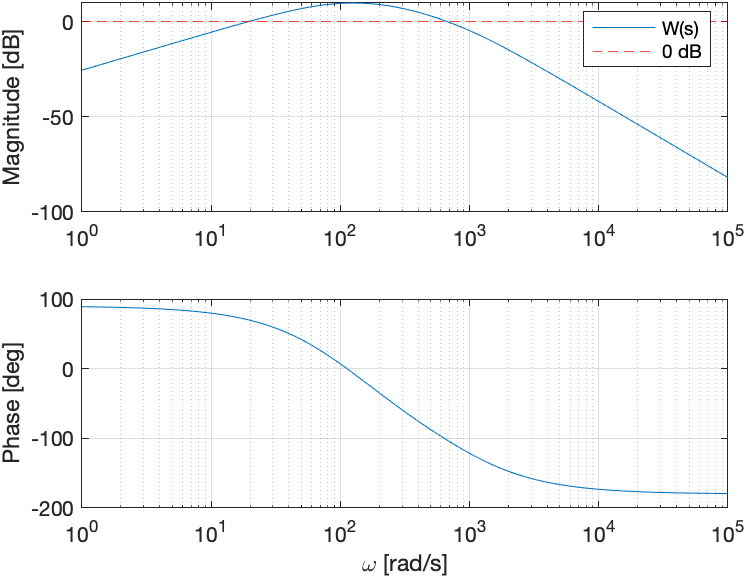
\includegraphics[height=250px]{../matlab/output/q2/c-iii}
	      	\captionof{figure}{Bode plot of $M(s)$  \label{fig:p2:c:ms}}
		}	
		
		As \Cref{fig:p2:c:ms} shown, the magnitude of $M(s)$ actually over the $0 \unit{dB}$ for some of the frequency. In short, the system is not robustly stable.
	\end{note}

	\begin{note}[iv) \Cref{note:p2:i} and \Cref{note:p2:iii} are not contradictory]{pink}{note:p2:iv}
		As discovered in \Cref{note:p2:i}, the system is stable for that particular case (as proved in \Cref{proof:p2}), but it does not necessarily mean the system is robustly stable for all cases (as \Cref{note:p2:iii} discovered). 
	\end{note}






%%%%%%%%%%%%%%%%%%%%%%%%%%%%%%%%%%%%%%%%%%%%%%%%%%%%%%%%%%%%%%%%%%%%%%%%%%%%%%%%
%% ************************************************************************** %%
%% *                      TODO [Remove For Final Copy!]                     * %%
%% ************************************************************************** %%
%%%%%%%%%%%%%%%%%%%%%%%%%%%%%%%%%%%%%%%%%%%%%%%%%%%%%%%%%%%%%%%%%%%%%%%%%%%%%%%%
%\printlistoftodos

%%%%%%%%%%%%%%%%%%%%%%%%%%%%%%%%%%%%%%%%%%%%%%%%%%%%%%%%%%%%%%%%%%%%%%%%%%%%%%%%
%% ************************************************************************** %%
%% *                                Glossary                                * %%
%% ************************************************************************** %%
%%%%%%%%%%%%%%%%%%%%%%%%%%%%%%%%%%%%%%%%%%%%%%%%%%%%%%%%%%%%%%%%%%%%%%%%%%%%%%%%
\clearpage
\printglossaries

%%%%%%%%%%%%%%%%%%%%%%%%%%%%%%%%%%%%%%%%%%%%%%%%%%%%%%%%%%%%%%%%%%%%%%%%%%%%%%%%
%% ************************************************************************** %%
%% *                               References                               * %%
%% ************************************************************************** %%
%%%%%%%%%%%%%%%%%%%%%%%%%%%%%%%%%%%%%%%%%%%%%%%%%%%%%%%%%%%%%%%%%%%%%%%%%%%%%%%%

% \printbibliography[heading=none]

%%%%%%%%%%%%%%%%%%%%%%%%%%%%%%%%%%%%%%%%%%%%%%%%%%%%%%%%%%%%%%%%%%%%%%%%%%%%%%%%
%% ************************************************************************** %%
%% *                               Appendices                               * %%
%% ************************************************************************** %%
%%%%%%%%%%%%%%%%%%%%%%%%%%%%%%%%%%%%%%%%%%%%%%%%%%%%%%%%%%%%%%%%%%%%%%%%%%%%%%%%
% appendices use section and subsection numbering
%\clearpage
\appendix
\begin{appendices}
% INPUT UR APPENDIX
\section{Code for Main}
\lstinputlisting[language=MATLAB, caption=Main Lab Contents, label=code:main]{../matlab/main.m}

\section{Code for Helper Class}
\lstinputlisting[language=MATLAB, caption=Helper and commonly used functions by main, label=code:helper]{../matlab/helper.m}

\end{appendices}

\end{document}


